\documentclass{beamer}
\usepackage[utf8]{inputenc}
\usetheme[background=dark,titleformat = smallcaps , block = fill,numbering = fraction, progressbar = 
frametitle , titleformat title= smallcaps]{metropolis}           % Use metropolis theme


\definecolor{orangeBar}{HTML}{FF3600}
\setbeamercolor{progress bar}{fg=orangeBar}

\usepackage{multimedia}
\usepackage{animate}
\usepackage {extarrows}
\usepackage {tikz}
\usepackage[options ]{algorithm2e}
\usepackage[spanish]{babel}
\usepackage{graphicx}
\usepackage{amssymb}
%\usepackage{amsfonts}

\usepackage{enumerate}
\usepackage{amsmath}
\usepackage{amsthm}
\usepackage{xcolor}
%\usepackage{amsfonts,amssymb,amsthm}

\usepackage{url}
\usepackage{enumerate}
\usepackage{commath}
\usepackage{multicol}
\usepackage{mathtools}
\usepackage{scrextend}
\usepackage{hyperref}
\usepackage{cleveref}
\usepackage{longtable}
\usepackage{bbm}
\usepackage{siunitx}
\usepackage{listings}
\usepackage{xcolor}
\usepackage{subcaption}
\usepackage{epigraph}
\usetikzlibrary{arrows}

\definecolor{codegreen}{rgb}{0,0.6,0}
\definecolor{codegray}{rgb}{0.5,0.5,0.5}
\definecolor{codepurple}{rgb}{0.58,0,0.82}
\definecolor{backcolour}{rgb}{0.95,0.95,0.92}
\definecolor{darkBlue}{HTML}{00000F}
\definecolor{lightBlue}{HTML}{00B7D4}
\definecolor{lightRed}{HTML}{E42525}
\definecolor{lightGreen}{HTML}{9CE425}

\definecolor{green0}{HTML}{B65900}
\definecolor{green1}{HTML}{D77200}
\definecolor{green2}{HTML}{ED8E30}
\definecolor{green3}{HTML}{FABE86}

\lstdefinestyle{mystyle}{
    backgroundcolor=\color{darkBlue},   
	commentstyle=\color{lightGreen},
	keywordstyle=\color{lightBlue},
	numberstyle=\tiny\color{codegray},
	stringstyle=\color{lightRed},
	basicstyle=\ttfamily\footnotesize,
	breakatwhitespace=false,         
	breaklines=true,                 
	captionpos=b,                    
	keepspaces=true,                 
	numbers=left,                    
	numbersep=5pt,                  
	showspaces=false,                
	showstringspaces=false,
	showtabs=false,                  
	tabsize=1
}

\lstset{style=mystyle}
\lstset{language=Python}
\lstset{frame=lines}
\lstset{caption={Insert code directly in your document}}
\lstset{label={lst:code_direct}}
\lstset{basicstyle=\footnotesize}


\newcommand{\bb}[1]{\mathbb{#1}}

%\newtheorem{theorem}{Teorema}[section]
%\theoremstyle{plain}
\newtheorem{acknowledgement}[theorem]{Acknowledgement}
%\newtheorem{algorithm}[theorem]{Algorithm}
\newtheorem{axiom}[theorem]{Axiom}
\newtheorem{case}[theorem]{Case}
\newtheorem{claim}{Claim}
\newtheorem{conclution}[theorem]{Conclusión}
\newtheorem{condition}[theorem]{Condition}
\newtheorem{conjecture}[theorem]{Conjecture}
%\newtheorem{corollary}[theorem]{Corolario}
\newtheorem{criterion}[theorem]{Criterion}
\theoremstyle{definition}
%\newtheorem*{df}{Definición}
%\newtheorem{definition}[theorem]{Definición}
%\newtheorem{example}[theorem]{Ejemplo}
\newtheorem{exercise}[theorem]{Exercise}
%\newtheorem{lemma}[theorem]{Lema}
\newtheorem{notation}[theorem]{Notation}
%\newtheorem{problem}[theorem]{Problem}
\newtheorem{proposition}[theorem]{Proposición}
\newtheorem{remark}[theorem]{Nota}
%\newtheorem{solution}[theorem]{Solución}
\newtheorem{summary}[theorem]{Summary}
\numberwithin{equation}{section}

\definecolor{defColor}{HTML}{3ED597}
\newcommand{\marine}[1]{\textcolor{defColor}{#1}}


\definecolor{thColor}{HTML}{FA7E0A}
\newcommand{\orangee}[1]{\textcolor{thColor}{#1}}

\definecolor{rkColor}{HTML}{F72121}
\newcommand{\redd}[1]{\textcolor{rkColor}{#1}}


%---------------emojis--------------------
\newcommand{\smiley}{\tikz[baseline=-0.75ex,black]{
		\draw circle (2mm);
		\node[fill,circle,inner sep=0.5pt] (left eye) at (135:0.8mm) {};
		\node[fill,circle,inner sep=0.5pt] (right eye) at (45:0.8mm) {};
		\draw (-145:0.9mm) arc (-120:-60:1.5mm);
	}
}

\newcommand{\frownie}{\tikz[baseline=-0.75ex,black]{
		\draw circle (2mm);
		\node[fill,circle,inner sep=0.5pt] (left eye) at (135:0.8mm) {};
		\node[fill,circle,inner sep=0.5pt] (right eye) at (45:0.8mm) {};
		\draw (-145:0.9mm) arc (120:60:1.5mm);
	}
}

\newcommand{\neutranie}{\tikz[baseline=-0.75ex,black]{
		\draw circle (2mm);
		\node[fill,circle,inner sep=0.5pt] (left eye) at (135:0.8mm) {};
		\node[fill,circle,inner sep=0.5pt] (right eye) at (45:0.8mm) {};
		\draw (-135:0.9mm) -- (-45:0.9mm);
	}
}




\newtheorem{df}{\marine{Definición}}
\newtheorem{thh}{\orangee{Teorema}}
\newtheorem{pr}{\orangee{Proposición}}
\newtheorem{lm}{\orangee{Lema}}
\newtheorem{crr}{\orangee{Corolario}}
\newtheorem{rr}{\redd{Observación}}
\usepackage{graphicx} 


%\newtheorem{defn}[]{Definición}
%\newenvironment{definition}{\begin{defn}}{\end{defn}}
%\newtheorem{definition}{Definition}[section]
%\newtheorem*{remark}{Remark}
%%%%%%%%
\newcommand{\tit}[1]{\textit{#1}}
\newcommand{\bsym}{\mathbf}
\newcommand{\Mod}[1]{\ (\mathrm{mod}\ #1)}
%\newcommand{\blue}[1]{\textcolor{blue}{#1}}
\newcommand{\red}[1]{\textcolor{red}{#1}}
\renewcommand{\geq}{\geqslant}
\renewcommand{\leq}{\leqslant}
\newcommand{\Rplus}{\mathds{R}_{^{+}}}
\newcommand{\N}{\mathbb{N}}
\newcommand{\Z}{\mathbb{Z}}
\newcommand{\R}{\mathbb{R}}

\newcommand{\C}{\mathbb{C}}
\newcommand{\Q}{\mathbb{Q}}
\newcommand{\ssi}{\longleftrightarrow}
\newcommand{\ent}{\longrightarrow}
\newcommand{\Qp}{\mathbb{Q}_p}  
\newcommand{\Qpn}{\mathbb{Q}_p^n}
\newcommand{\Zpn}{\mathbb{Z}_p^n}
\newcommand{\Zp}{\mathbb{Z}_p}
\newcommand{\Zd}{\mathbb{Z}_2}
%\newcommand{\abs}[1]{\left\vert #1 \right\vert}
%\newcommand{\norm}[1]{\|#1\|}
\newcommand{\pnorm}[1]{\|#1\|_p}
\newcommand{\maxx}[1]{\text{m\'ax} #1}
\newcommand{\xbar}[1]{\hskip 1.4pt\overline{\hskip-1.2pt #1\hskip -.6pt}\hskip 1.2pt}
\newcommand{\rb}{\raisebox{-.35ex}}

\DeclareMathOperator{\s}{\mathbf{S}}
\DeclareMathOperator{\f}{\mathcal{F}}
\DeclareMathOperator{\A}{\mathbb{A}}
\DeclareMathOperator{\dist}{dist} % The distance.
\DeclareMathOperator{\d^n}{\dif^{\,n}}
%\DeclareMathOperator{\d}{\dif}
\DeclareMathOperator{\Real}{Re}
\DeclareMathOperator{\ord}{Ord}
\DeclareMathOperator{\Dom}{Dom}
\DeclareMathOperator{\vol}{vol}
\DeclareMathOperator{\gpn}{\mathit{{GpnN}}}
%%%%%%%%%
%%%%%%%%%%%%%%%%% dashed integrals %%%%%%%%%%%%%%%%%%%%%
\DeclareSymbolFont{eulargesymbols}{U}{zeuex}{m}{n}
\DeclareMathSymbol{\intop}{\mathop}{eulargesymbols}{"52}
\usepackage[toc,page]{appendix}
\renewcommand{\labelitemi}{$\circ$}


\title{Análisis de la infraestructura turística de las principales ciudades del país}
\subtitle{Proyecto final, Estadística Multivariada}
\date{27 de Mayo de 2021}


\author{\bf{Autores: }Edgar Baquero \& Enrique Santibáñez}

\institute{Centro de Investigación en Matemáticas, \\Maestría en Cómputo Estadístico.}
%Facultad de Ciencias\\
%Departamento de Matemáticas}



\usepackage{MnSymbol,wasysym}



\titlegraphic{%
	\begin{picture}(0,0)
	\put(190,-190){\makebox(0,0)[rt]{
\includegraphics[width=2cm]{logo}}}
    \end{picture}
}

\usepackage[backend=biber, style=apa, natbib = true]{biblatex}
\bibliography{biblio.bib}
\begin{document}
  \maketitle

\begin{frame}{Contenido}
	\tableofcontents
\end{frame}

\section{Importancia y Objetivo del proyecto}
\begin{frame}{Importancia y Objetivo del proyecto}
	
	\begin{enumerate}[<+- | alert@+>]
	    \item Visualizar la infraestructura ciudades principales de México
	    \item Usar técnicas multivariadas
	    \item Escalar los datos factíblemente
	    \item Analizar la demanda (Llegada de turistas y ocupación)
	    \item Analizar la oferta (Infraestructura turística)
	    \item Definir una medida de similaridad apropiada entre ciudades
	    \item Reconocer grupos de ciudades
	\end{enumerate}
\end{frame}
\section{Metodología}

\begin{frame}{Metodología, MDS}
	
	\begin{enumerate}
	[<+- | alert@+>]
	    \item Queremos una representación en $q\leq N - 1$ dimensiones
	    \item Hay $M = \frac{N(N-1)}{2}$ similaridades 
	    \item Suponiendo un orden:
	    $$
        s_{i_{1} k_{1}}<s_{i_{2} k_{2}}<\cdots<s_{i_{M} k_{M}}
        $$
        \item En la nueva representación queremos preservar:
        $$
d_{i_{1} k_{1}}^{(q)}>d_{i_{2} k_{2}}^{(q)}>\cdots>d_{i_Mk_M}^{(q)}
$$
\item Evaluaremos a través de la medida de Stress (Kruskal, 1964):
$$
Stress(q)=\left\{\frac{\sum_{i<k}\left(d_{i k}^{(q)}-\hat{d}_{i k}^{(q)}\right)^{2}}{\sum_{i<k}\left[d_{i k}^{(q)}\right]^{2}}\right\}^{1/2}
$$
	    
	\end{enumerate}
\end{frame}

\begin{frame}{Metodología, MDS}
	La evaluación (según Kruskal) del Stress se puede interpretar a través:
	\begin{center}
\begin{tabular}{r l}
Stress & Ajuste \\
\hline
20\% & pobre \\
10\% & normal \\
5\% & bueno\\
2.5\% & Excelente\\
0\% & Perfecto
\end{tabular}
\end{center}
Usamos la solución por Coordenadas principales.
\end{frame}

\begin{frame}{Metodología, Selección de similaridad}
Presentamos 3 tipos de similaridad calculables para los datos originales:
	
\begin{enumerate}
	[<+- | alert@+>]
	    \item Similaridad Euclideana:
	    $$s_{ij} = \sqrt{\sum_{k=1}^N(c_{ik}-c_{jk})^2 }$$
	    \item Similaridad Coseno:
	    $$
    s_{ij}=\operatorname{cos} \theta_{ij}=\frac{\vec{c_j} \cdot \vec{c_j}}{\|\vec{c_i}\|\|\vec{c_j}\|}=\frac{\sum_{1}^{n} c_i_{k} c_j_{k}}{\sqrt{\sum_{1}^{n} c_i_{k}^{2}} \sqrt{\sum_{1}^{n} c_j_{k}^{2}}}
    $$
    \item Similaridad de \textit{Coxon} \citep{mds_book_ref}:
    \begin{align} \label{coxon}
    s_{ij}=\sqrt{2(1-r_{ij})}
    \end{align}
    
\end{enumerate}

    
\end{frame}

\begin{frame}{Metodología, Cústering}
Dado que hay $N = 37$ ciudades. parece conveniente representarlas en jerarquías
\begin{enumerate}
	[<+- | alert@+>]
	    \item Datos originales $\Longrightarrow$ Clústering Jerárquico
	    \item Matriz de distancias $\Longrightarrow$ Clústering por $K$-Means
    
\end{enumerate}

    
\end{frame}




\begin{frame}{Metodología, Cústering}
\begin{algorithm}[H]
\SetAlgoLined
\KwResult{conjunto de centroides}
 \While{La asignación de clústeres cambie}{
  Para alguna asignación de clúster, $C$, la varianza es minimizada respecto a $\{m_1,\dots,m_K\}$, llevando a la media del cluster asignado\;
  
  Dado el conjunto $\{m_1,\dots,m_K\}$, minimizamos
$  
\min _{C,\left\{m_{k}\right\}_{1}^{K}} \sum_{k=1}^{K} N_{k} \sum_{C(i)=k}\left\|x_{i}-m_{k}\right\|^{2}
$, asignando cada observación a su cluster más cercano:\;
$$
C(i)=\operatorname{argmin}_{1 \leq k \leq K}\left\|x_{i}-m_{k}\right\|^{2}
$$
 }
 \caption{$K$-means Clústering}
\end{algorithm}

    
\end{frame}



\section{Descripción de las fuentes de información}
\subsection{Oferta turística}
\begin{frame}{Estructura de la oferta turística}
Consideramos que la oferta turística de una ciudad se define por los servicios que cuenta cada ciudad para generar atracciones o comodidad a los turistas.
    \begin{figure}
        \centering
        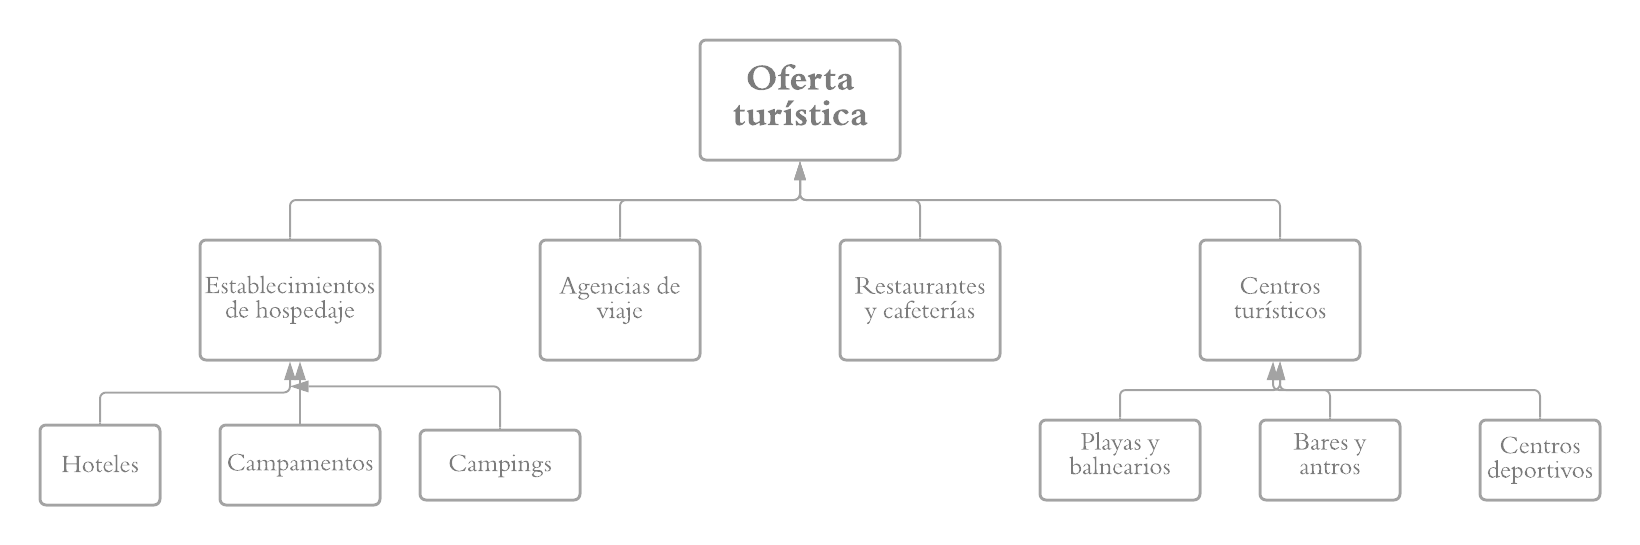
\includegraphics[scale=0.2]{figure/diagrama_oferta.png}
        \caption{Estructura de la oferta turística}
        \label{fig:diagrama_oferta}
    \end{figure}
\end{frame}
\begin{frame}{Información de la oferta turística}
    Los datos se han obtenido del Directorio Estadístico Nacional de Unidades Económicas 2019 (DE-NUE) que realiza el Instituto Nacional de Estadística y Geografía (INEGI) \citep{denue}.
    \begin{figure}
        \centering
        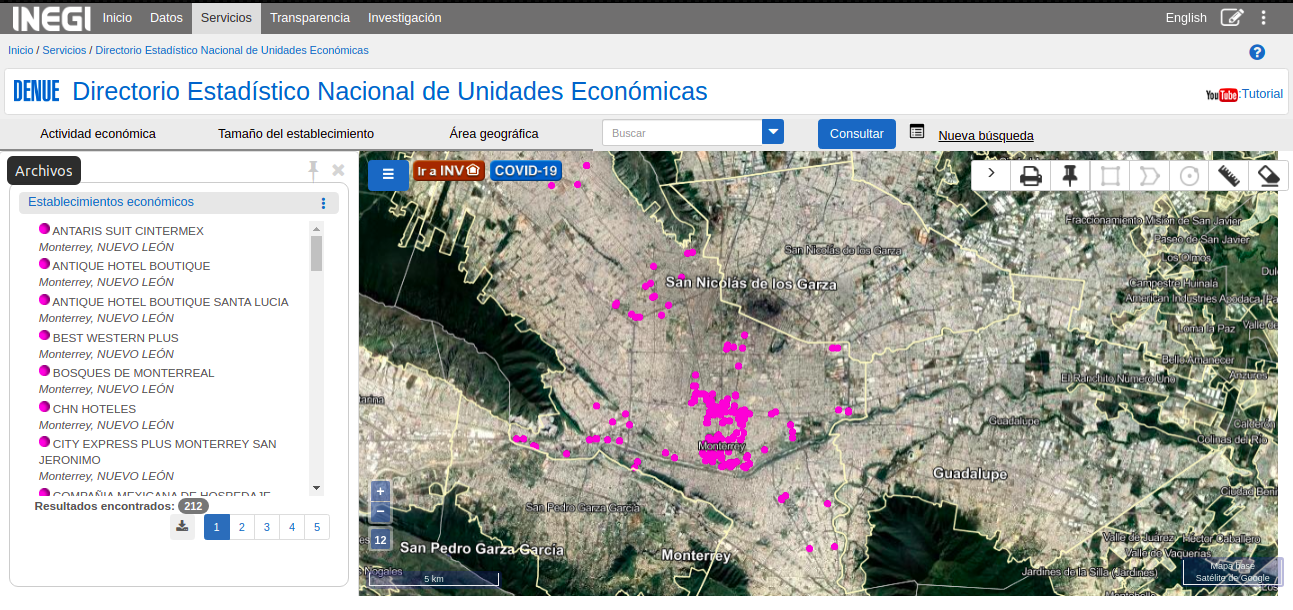
\includegraphics[scale=0.22]{figure/denue_mapa_interactivo.png}
        \caption{Map interactivo DENUE}
        \label{fig:denue_mapa_interactivo}
    \end{figure}
\end{frame}

\subsection{Demanda turística}
\begin{frame}{Estructura de la demanda turística}
    Para medir la demanda turística de cada ciudad, lo ideal sería tener el dato real de cuantos turistas existen por ciudad. Pero un \textit{proxy} de este valor es considerar los registros hoteleros y de los centros turísticos.
    \begin{figure}
        \centering
        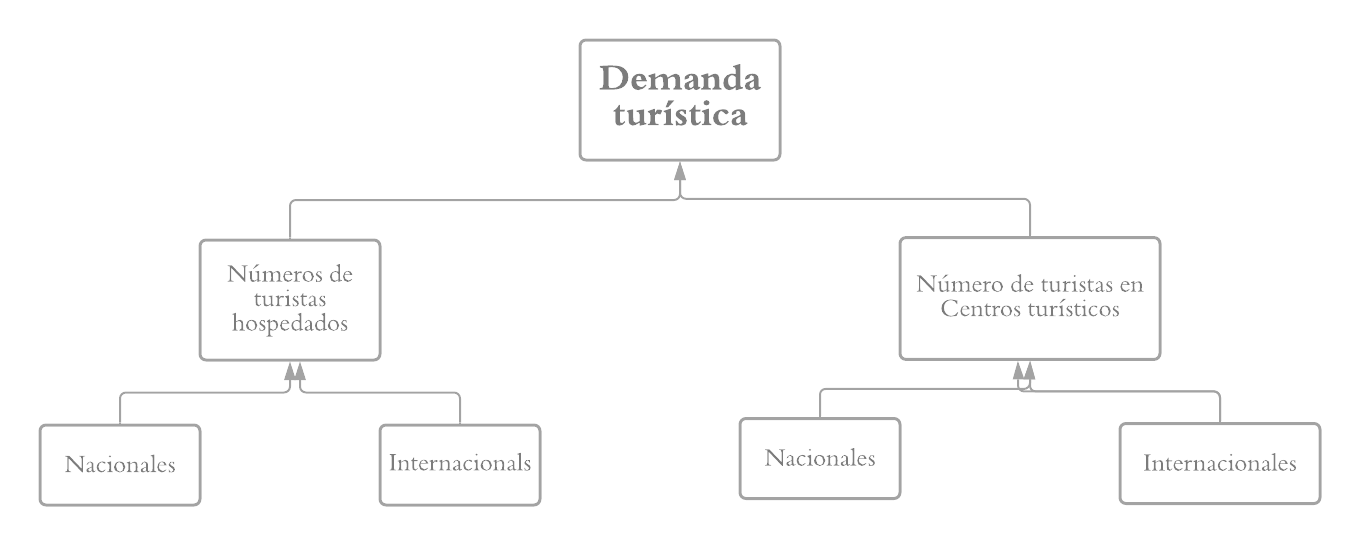
\includegraphics[scale=0.22]{figure/diagrama_demanda.png}
        \caption{Estructura de la demanda turística}
        \label{fig:diagrama_demanda}
    \end{figure}
\end{frame}

\begin{frame}{Información de la demanda turística.}
    El Monitoreo Hotelero Data-Tur reúne información estadística de las principales variables como flujo de viajeros internacionales, turismo doméstico, flujos aéreos y marítimos, actividades de alojamiento, las cuales en su conjunto ofrecen una perspectiva de la dinámica del sector turismo en México \citep{datatour}.
    \begin{figure}
        \centering
        
\includegraphics[scale=.6]{figure/datatur.png}
        \caption{Logo Datatur}
        \label{fig:datatur}
    \end{figure}
\end{frame}

\section{Resultados}

\begin{frame}{Oferta hotelera}
\begin{figure}
    \centering
    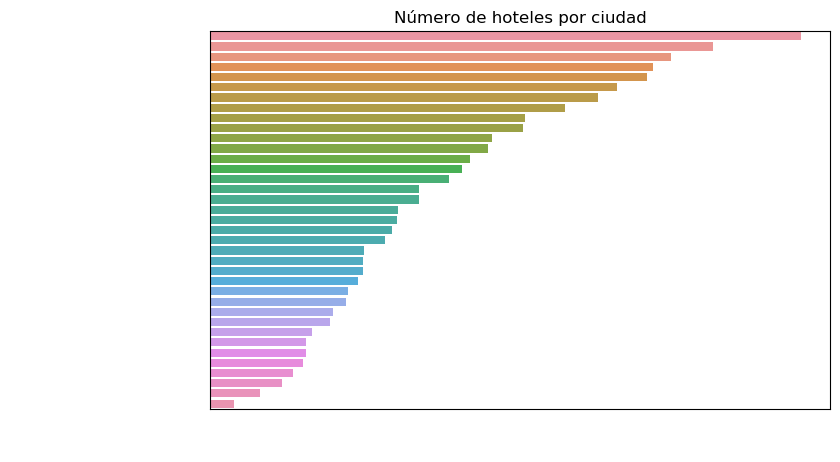
\includegraphics[scale=0.5]{figure/hoteles.png}
    \caption{Distribución de la cantidad de hoteles por ciudad}
    \label{fig:hoteles}
\end{figure}
\end{frame}

\begin{frame}{Agencias de viaje}
\begin{figure}
    \centering
    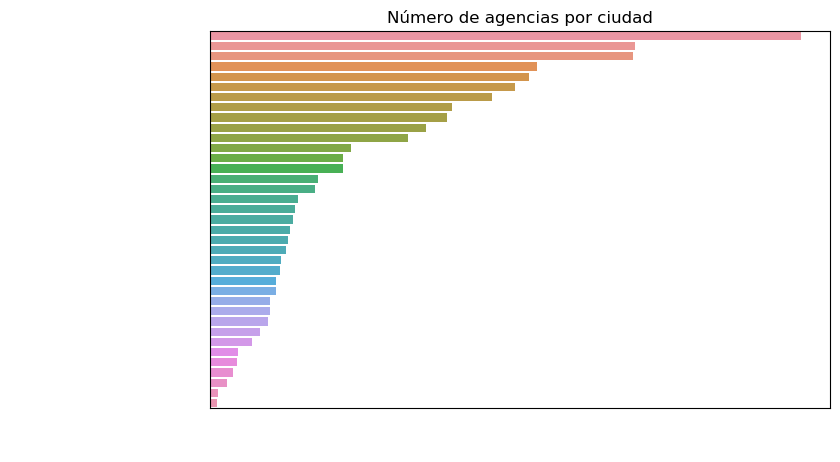
\includegraphics[scale=0.5]{figure/agencias.png}
    \caption{Distribución de la cantidad de agencias de viajes por ciudad}
    \label{fig:agencias}
\end{figure}
\end{frame}

\begin{frame}{Restaurantes, cafetería y fondas.}
\begin{figure}
    \centering
    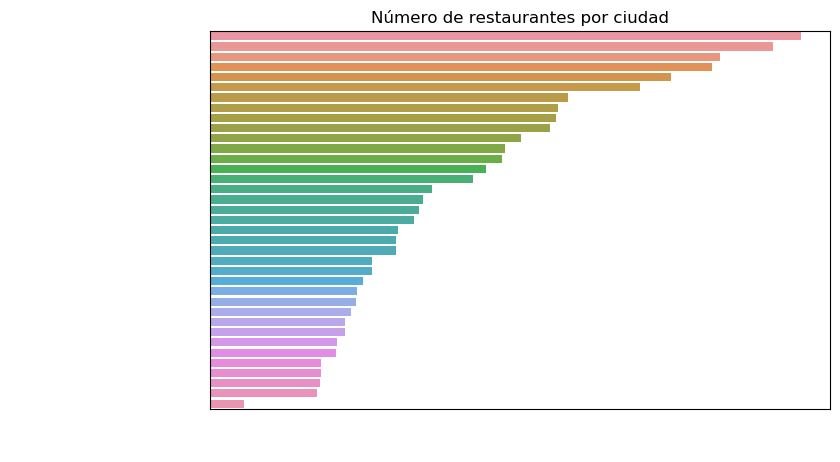
\includegraphics[scale=0.5]{figure/restaurantes.png}
    \caption{Distribución de la cantidad de servicios de comida por ciudad}
    \label{fig:restaurantes}
\end{figure}
\end{frame}

\begin{frame}{Lugares de ocio y recreativos}
    \begin{figure}
        \centering
        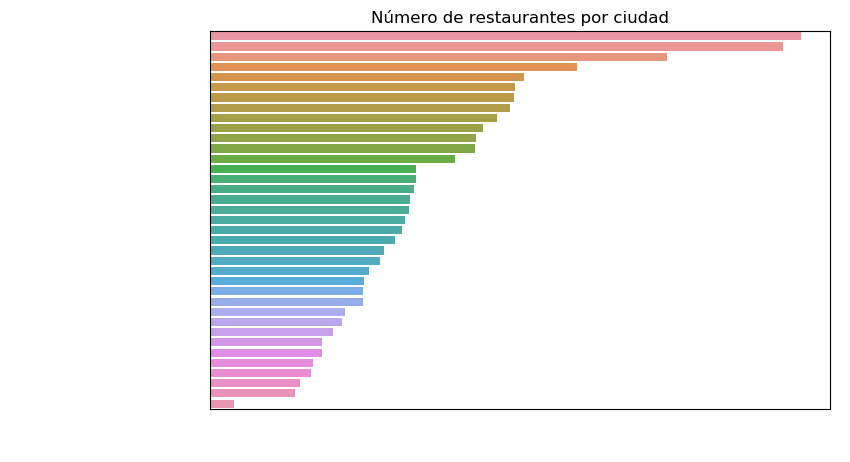
\includegraphics[scale=0.5]{figure/ocio.png}
        \caption{Distribución de la cantidad de lugares de ocio y recreativos por ciudad}
        \label{fig:ocio}
    \end{figure}
\end{frame}

\begin{frame}{Turistas extrajeros}
\begin{figure}
    \centering
    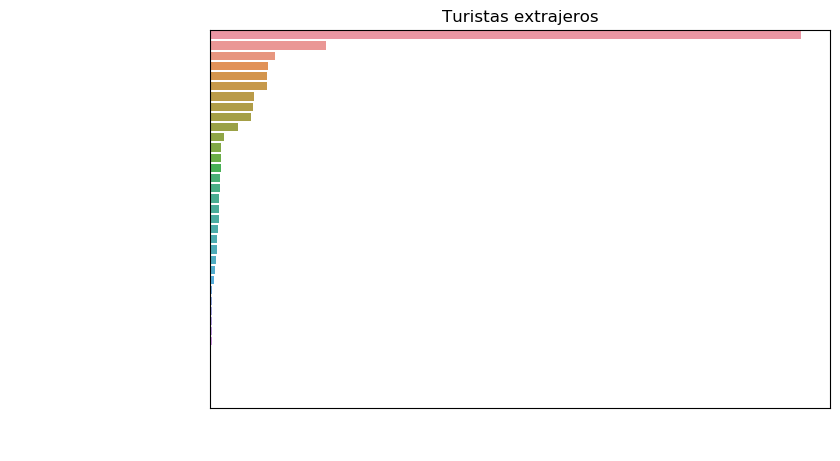
\includegraphics[scale=0.5]{figure/turistas_extranjeros.png}
    \caption{Turistas extrajeros}
    \label{fig:turistas_extranjeros}
\end{figure}
\end{frame}

\begin{frame}{Turistas nacionales}
\begin{figure}
    \centering
    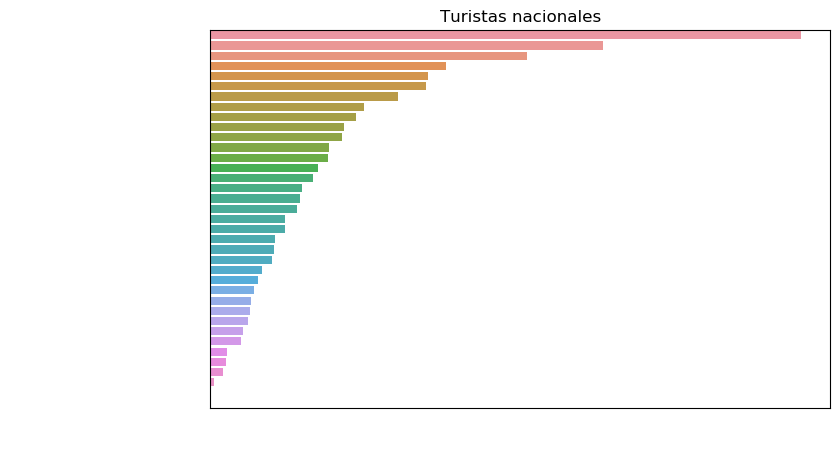
\includegraphics[scale=0.5]{figure/turistas_nacionales.png}
    \caption{Turistas nacionales}
    \label{fig:turistas_nacionales}
\end{figure}
\end{frame}




\begin{frame}{Oferta turística}
    \begin{itemize}[<+- | alert@+>]
\item Para determinar las proximidades que existen entre las ciudades, consideremos la distancia euclidiana como primer enfoque. Pero esta medida de distancia no arrojaba buenos resultados. 

\item En un estudio similar \cite{mds_tur}, utilizaron una medida de disimilaridad para cada par de observaciones mediante el coeficiente de correlación. 

\item Considerando la transformación de Coxon (1) a partir de los datos obtenidos del DENUE hemos aplicado MDS, obteniendo la configuración de la Figura \ref{fig:oferta_turistica_c}.
	\end{itemize}
\end{frame}

\begin{frame}{Configuración MDS}
    El STRESS obtenido es de 0.1034, lo cual nos indica que el ajuste de los datos es regular. 
        \begin{figure}
        \centering
        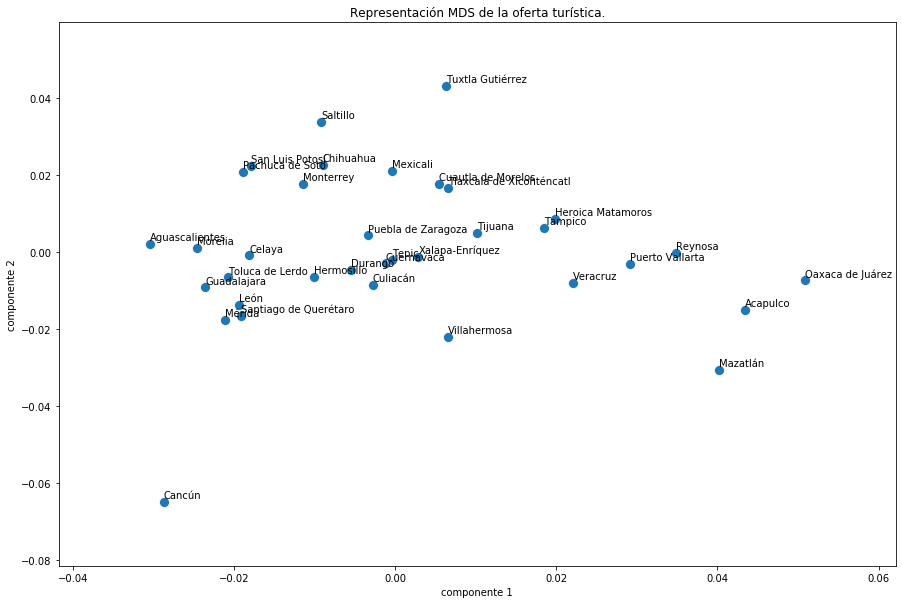
\includegraphics[scale=0.28]{figure/oferta_turistica_c.png}
        \caption{Configuración MDS}
        \label{fig:oferta_turistica_c}
    \end{figure}
\end{frame}


\begin{frame}{Demanda turística}
    \begin{itemize}[<+- | alert@+>]
        \item El segundo objetivo de este trabajo es determinar la demanda turística de cada ciudad. Para ello,con ayuda de los datos recabados de Datatur procedimos a realizar el análogo a lo que se hizo en oferta turística.
        
        \item     En este caso, la configuración obtenido con MDS tuvo mejores resultados (Ver Figura 8). Obtuvimosun STRESS de 0.01, lo que nos indica que el ajuste es muy bueno. 
    \end{itemize}
\end{frame}

\begin{frame}{Configuración MDS, demanda turística}
        \begin{figure}
        \centering
        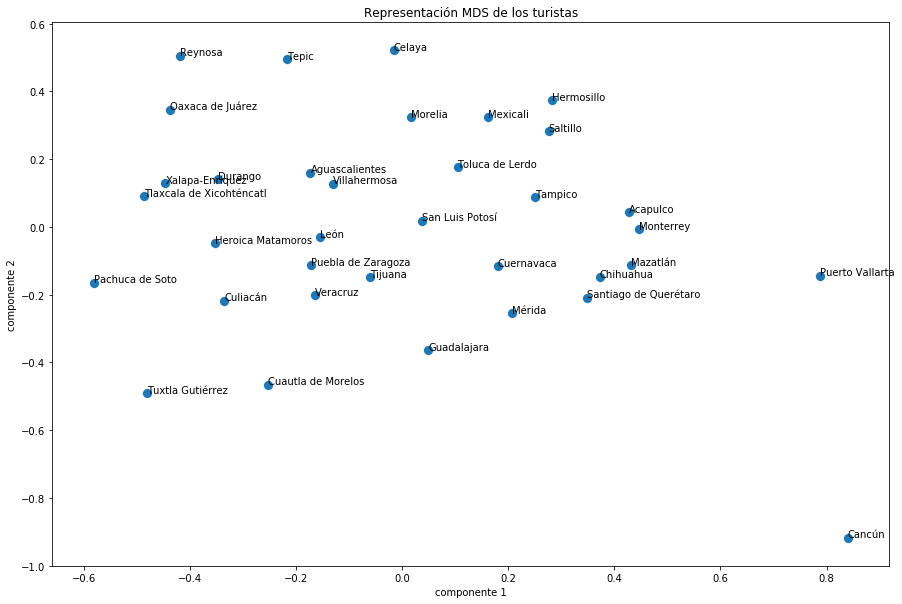
\includegraphics[scale=.335]{figure/demanda_turistica_c.png}
        \caption{Configuración MDS, demanda turística}
        \label{fig:demanda_turistica_c}
    \end{figure}
\end{frame}

\section{Intepretación de resultados}
\begin{frame}{Comparación de clustering y las configuración MDS}
    La última parte de este trabajo es comparar los métodos de clustering KMeans y Métodos jerárquicos, con la configuración obtenida en MDS. Para ello, 
    \begin{itemize}
        \item ocupamos métodos conglomerados a los datos originales de oferta y demanda.
        
        \item ocupamos KMeans a la matriz de distancias de la transformación Coxon de la matriz de correlación entre las ciudades. 
    \end{itemize}
\end{frame}

\begin{frame}{Clustering oferta usando KNN}
    \begin{figure}
        \centering
        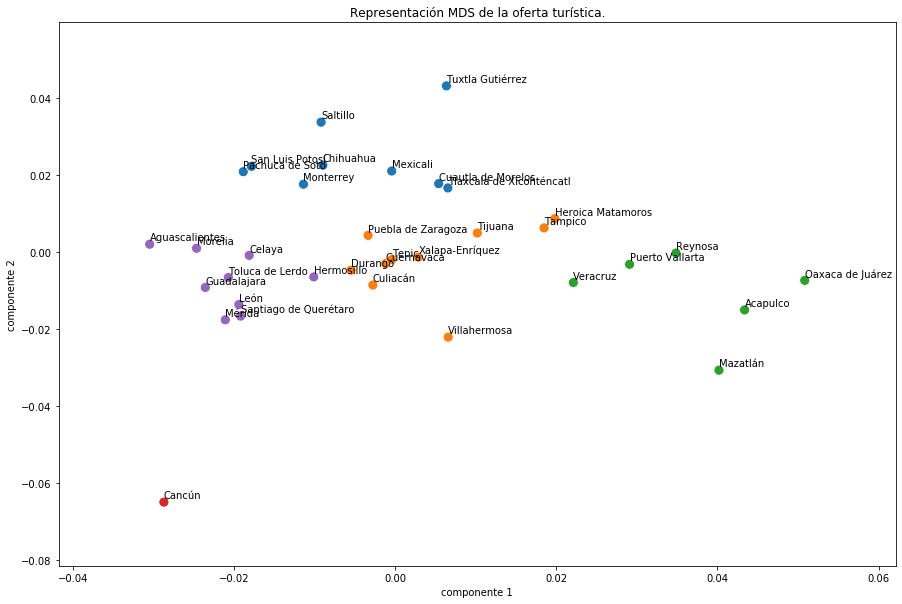
\includegraphics[scale=0.335]{figure/knn_oferta_c.png}
        \caption{KNN a la matriz de distancias}
        \label{fig:knn_oferta_c}
    \end{figure}
\end{frame}

\begin{frame}{Clustering oferta usando conglomerados}
    \begin{figure}
        \centering
        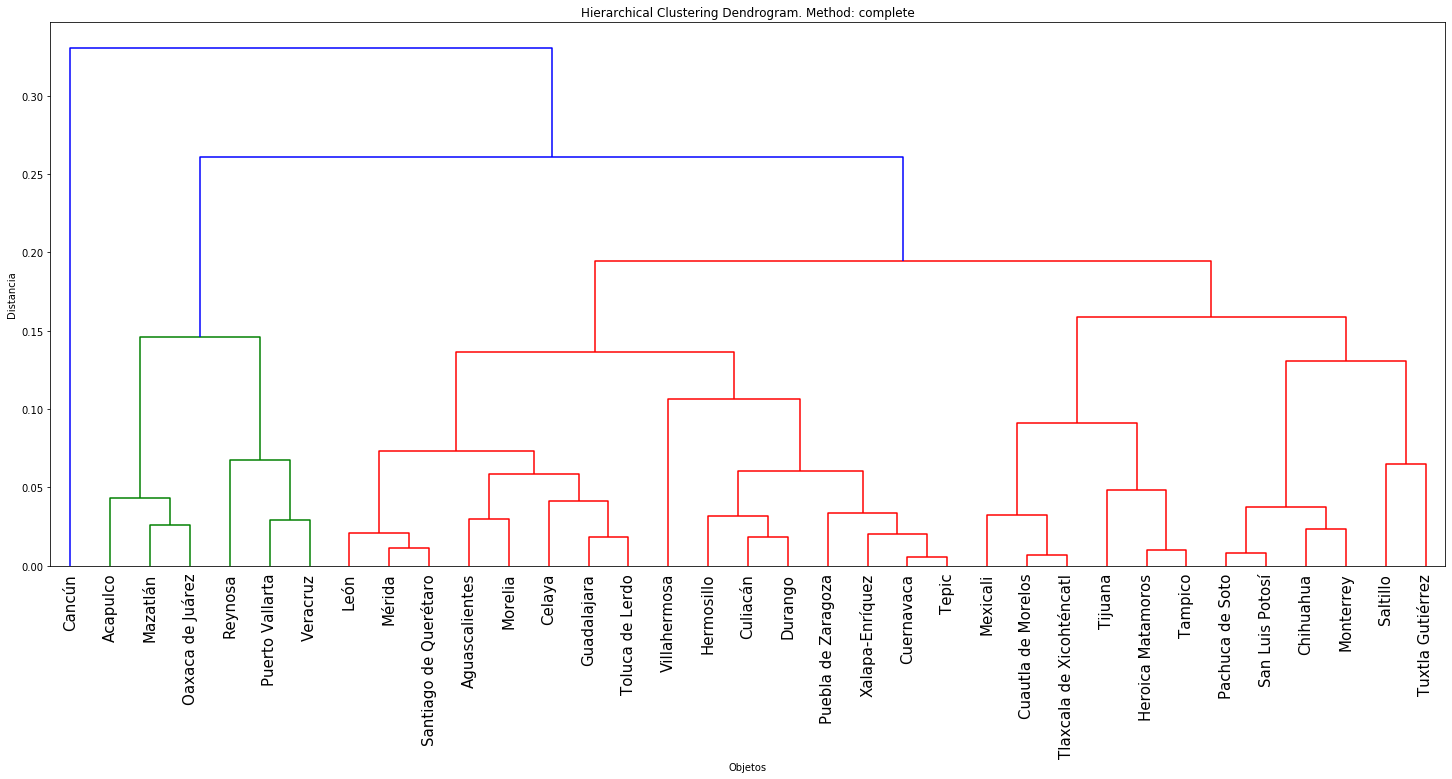
\includegraphics[scale=0.22]{figure/herarquico_oferta_c.png}
        \caption{Análisis de Conglomerados a la matriz de datos.}
        \label{fig:knn_oferta_c}
    \end{figure}
\end{frame}


\begin{frame}{Clustering demanda usando KNN}
    \begin{figure}
        \centering
        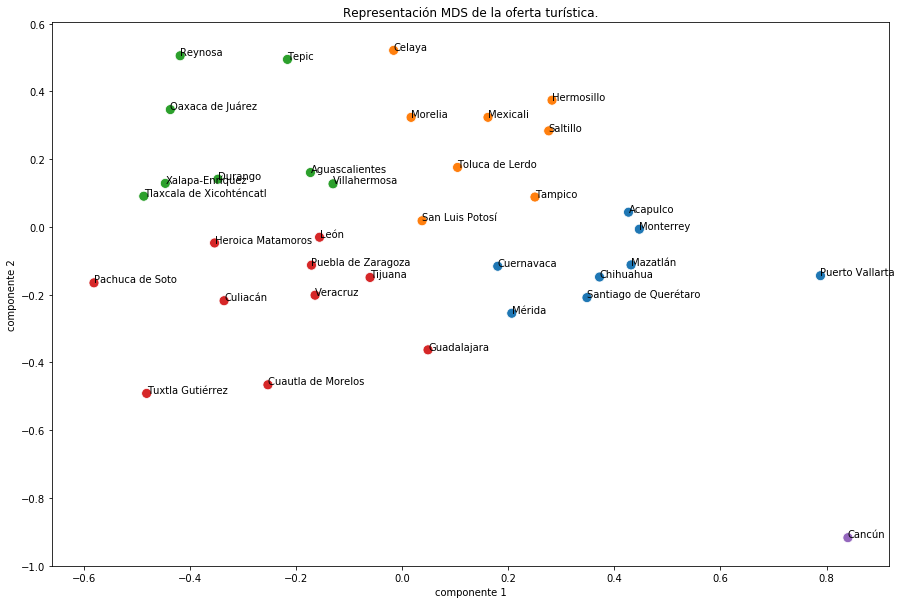
\includegraphics[scale=0.335]{figure/knn_demanda_c.png}
        \caption{KNN a la matriz de distancias}
        \label{fig:knn_demanda_c}
    \end{figure}
\end{frame}

\begin{frame}{Clustering demanda usando conglomerados}
    \begin{figure}
        \centering
        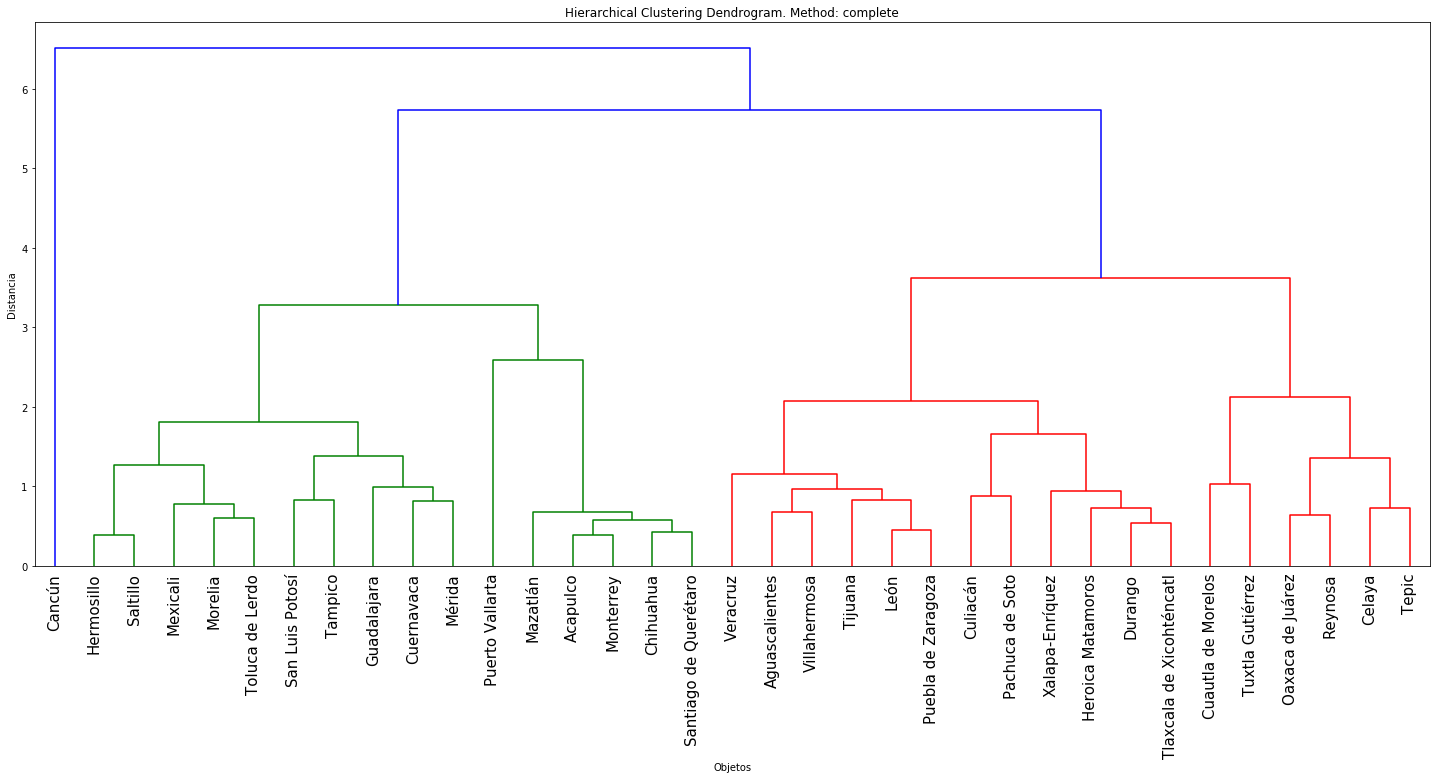
\includegraphics[scale=0.22]{figure/herarquico_demanda_c.png}
        \caption{Análisis de Conglomerados a la matriz de datos.}
        \label{fig:knn_oferta_c}
    \end{figure}
\end{frame}



\section{Conclusiones}
\begin{frame}

\begin{itemize}
    \item En conclusión  podemos decir que ambas configuraciones de la demanda y la oferta turística fueron buenas, pero la demanda tuvo mejores resultados poder tener una interpretación de los componentes que los de la oferta. 
    
    \item Además podemos concluir que las configuraciones obtenidas presentan muy buenos resultados comparados con los métodos de clustering no supervisado.
\end{itemize}
\end{frame}


\section*{Gracias \blacksmiley{}}

\printbibliography


\end{document}